\begin{pastexam}[label={px:gk3-113-ds-01}]{高考三級資訊處理 113 年 第一題}
（申論；25 分）

\begin{itemize}[leftmargin=2.2em]
\item[㈠] 若有 200 人，其中一個人開始打電話給兩個人。隨後，每個接到電話的人都會打電話給另外兩個尚沒有
接到電話的人。請問總共會撥打多少通電話？有多少人不會打電話？（無推導過程不給分）（10 分）
\item[㈡] 若一個二元樹其前序追蹤順序（Preorder Traversal）及後序追蹤順序（Postorder Traversal）分別如下，
請問此樹是否唯一？並請列出此二元樹的中序追蹤順序（Inorder Traversal）。（無推導過程不給分）（15 分）

前序追蹤順序：T, S, R, F, D, I, H, E, Z, G, M, L, J, N, Q\\
後序追蹤順序：F, I, H, D, R, Z, G, E, S, J, N, L, Q, M, T
\end{itemize}
\end{pastexam}

\begin{pastsoln}
答案：㈠ 共 $199$ 通電話，$100$ 人不會打電話。 ㈡ 唯一；中序是 F, R, I, D, H, S, Z, E, G, T, J, L, N, M, Q。

\textbf{㈠} 把每個人當成一個節點，「$a$ 打給 $b$」就讓 $b$ 成為 $a$ 的子節點。 每個人只會接到一次電話
（只打給還沒接到電話的人），第一個人不接電話，所以這 $200$ 人構成一棵以第一個人為根的樹，每通電話
是一條邊。
\begin{itemize}
\item \textbf{電話數}：除了根，每個人恰好接到一通電話，所以電話數＝邊數＝$200 - 1 = 199$ 通。
（只要還有人沒接到電話，就還有接到電話的人要往下打，所以最後 $200$ 人都會接到。）
\item \textbf{不打電話的人}：每個打電話的人打 $2$ 通，但 $199$ 是奇數，所以一定有一個人只打了 $1$ 通——
輪到他打的時候只剩一個人還沒接到電話。 設打 $2$ 通的有 $n_2$ 人、打 $1$ 通的有 $n_1$ 人、不打的有
$n_0$ 人：
\[
2n_2 + n_1 = 199,\qquad n_1 = 1 \ \Rightarrow\ n_2 = 99,\qquad n_0 = 200 - 99 - 1 = 100.
\]
也可以用資結書定理~7.2 的 $n_0 = n_2 + 1 = 100$ 驗證。 這棵樹就是 $200$ 個節點的完整二元樹（依接到
電話的先後編號 $1 \sim 200$，第 $i$ 人打給第 $2i$、$2i+1$ 人），編號 $101 \sim 200$ 的 $100$ 人是葉子，
不打電話；第 $100$ 人只打給第 $200$ 人。
\end{itemize}

\textbf{㈡ 重建。} 前序的第一個、後序的最後一個是根。 根之後前序的下一個是左子樹的根 $a$；在後序裡找到
$a$，$a$ 和它前面的部分就是整個左子樹，其餘是右子樹（資結書第~7.4~節）。 逐層拆：
\begin{itemize}
\item 根 $T$。 左子樹根 $S$，在後序中是第 $9$ 個，所以左子樹有 $9$ 個節點：
前序 $S\,R\,F\,D\,I\,H\,E\,Z\,G$、後序 $F\,I\,H\,D\,R\,Z\,G\,E\,S$；右子樹前序 $M\,L\,J\,N\,Q$、後序
$J\,N\,L\,Q\,M$。
\item $S$ 的左子樹根 $R$，後序第 $5$ 個：$R$ 子樹前序 $R\,F\,D\,I\,H$、後序 $F\,I\,H\,D\,R$；$S$ 的右
子樹前序 $E\,Z\,G$、後序 $Z\,G\,E$。
\item $R$：左子樹根 $F$，後序第 $1$ 個，只有 $F$；右子樹前序 $D\,I\,H$、後序 $I\,H\,D$，是 $D$ 帶左
子 $I$、右子 $H$。
\item $E$：前序 $Z\,G$、後序 $Z\,G$，左子 $Z$、右子 $G$。
\item $M$：左子樹根 $L$，後序 $J\,N\,L$ 共 $3$ 個，是 $L$ 帶左子 $J$、右子 $N$；右子樹只有 $Q$。
\end{itemize}
\begin{center}
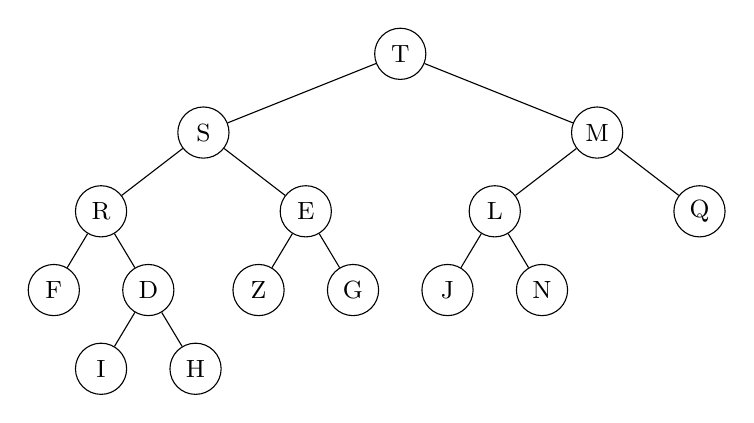
\begin{tikzpicture}[every node/.style={circle,draw,minimum size=6.5mm,inner sep=0pt,font=\small},
  level distance=10mm, level 1/.style={sibling distance=50mm}, level 2/.style={sibling distance=26mm},
  level 3/.style={sibling distance=12mm}]
\node {T}
  child {node {S}
    child {node {R} child {node {F}} child {node {D} child {node {I}} child {node {H}}}}
    child {node {E} child {node {Z}} child {node {G}}}}
  child {node {M}
    child {node {L} child {node {J}} child {node {N}}}
    child {node {Q}}};
\end{tikzpicture}
\end{center}

\textbf{唯一性。} 一般來說前序加後序不能決定二元樹：一個節點只有一個子節點時，看不出那個子節點在左
還是右（資結書定理~7.5：符合的樹有 $2^m$ 棵，$m$ 是只有一個子節點的節點數）。 上面每一步拆出的左右
子樹都非空——每個內部節點 $T, S, R, D, E, M, L$ 都恰有兩個子節點，$m = 0$，所以這棵樹是嚴格二元樹
（$7$ 個內部節點、$8$ 個葉子，$n_0 = n_2 + 1$），符合的樹只有 $2^0 = 1$ 棵，\textbf{唯一}。

\textbf{中序}（左、根、右）：$R$ 子樹是 $F\,R\,I\,D\,H$，$E$ 子樹是 $Z\,E\,G$，所以 $S$ 子樹是
$F\,R\,I\,D\,H\,S\,Z\,E\,G$；$M$ 子樹是 $J\,L\,N\,M\,Q$。 整棵樹：
\[
F, R, I, D, H, S, Z, E, G, T, J, L, N, M, Q.
\]
把這棵樹再做一次前序、後序，和題目給的完全一樣。
\end{pastsoln}
